\begin{frame}{GNU/Linux prima delle distribuzioni}
    \begin{itemize}
        \item Linux era distribuito solo come codice sorgente
        \item Chi voleva usare Linux doveva compilarlo da sé
        \item L'utilizzo era quindi accessibile solo agli sviluppatori
    \end{itemize}
    \hfill \break
    Per semplificare il processo di installazione e configurazione nascono le distribuzioni GNU/Linux.
\end{frame}

%------------------------------------------------

\begin{frame}{Le prime distribuzioni GNU/Linux}
    \begin{itemize}
        \item Boot-root - fine 1991
        \item MCC Interim Linux - 1992
        \item Slackware - 1993
        \item Yggdrasil Linux (Plug-and-Play) - 1993
    \end{itemize}
\end{frame}

\begin{frame}{Boot-root}
    \centering
    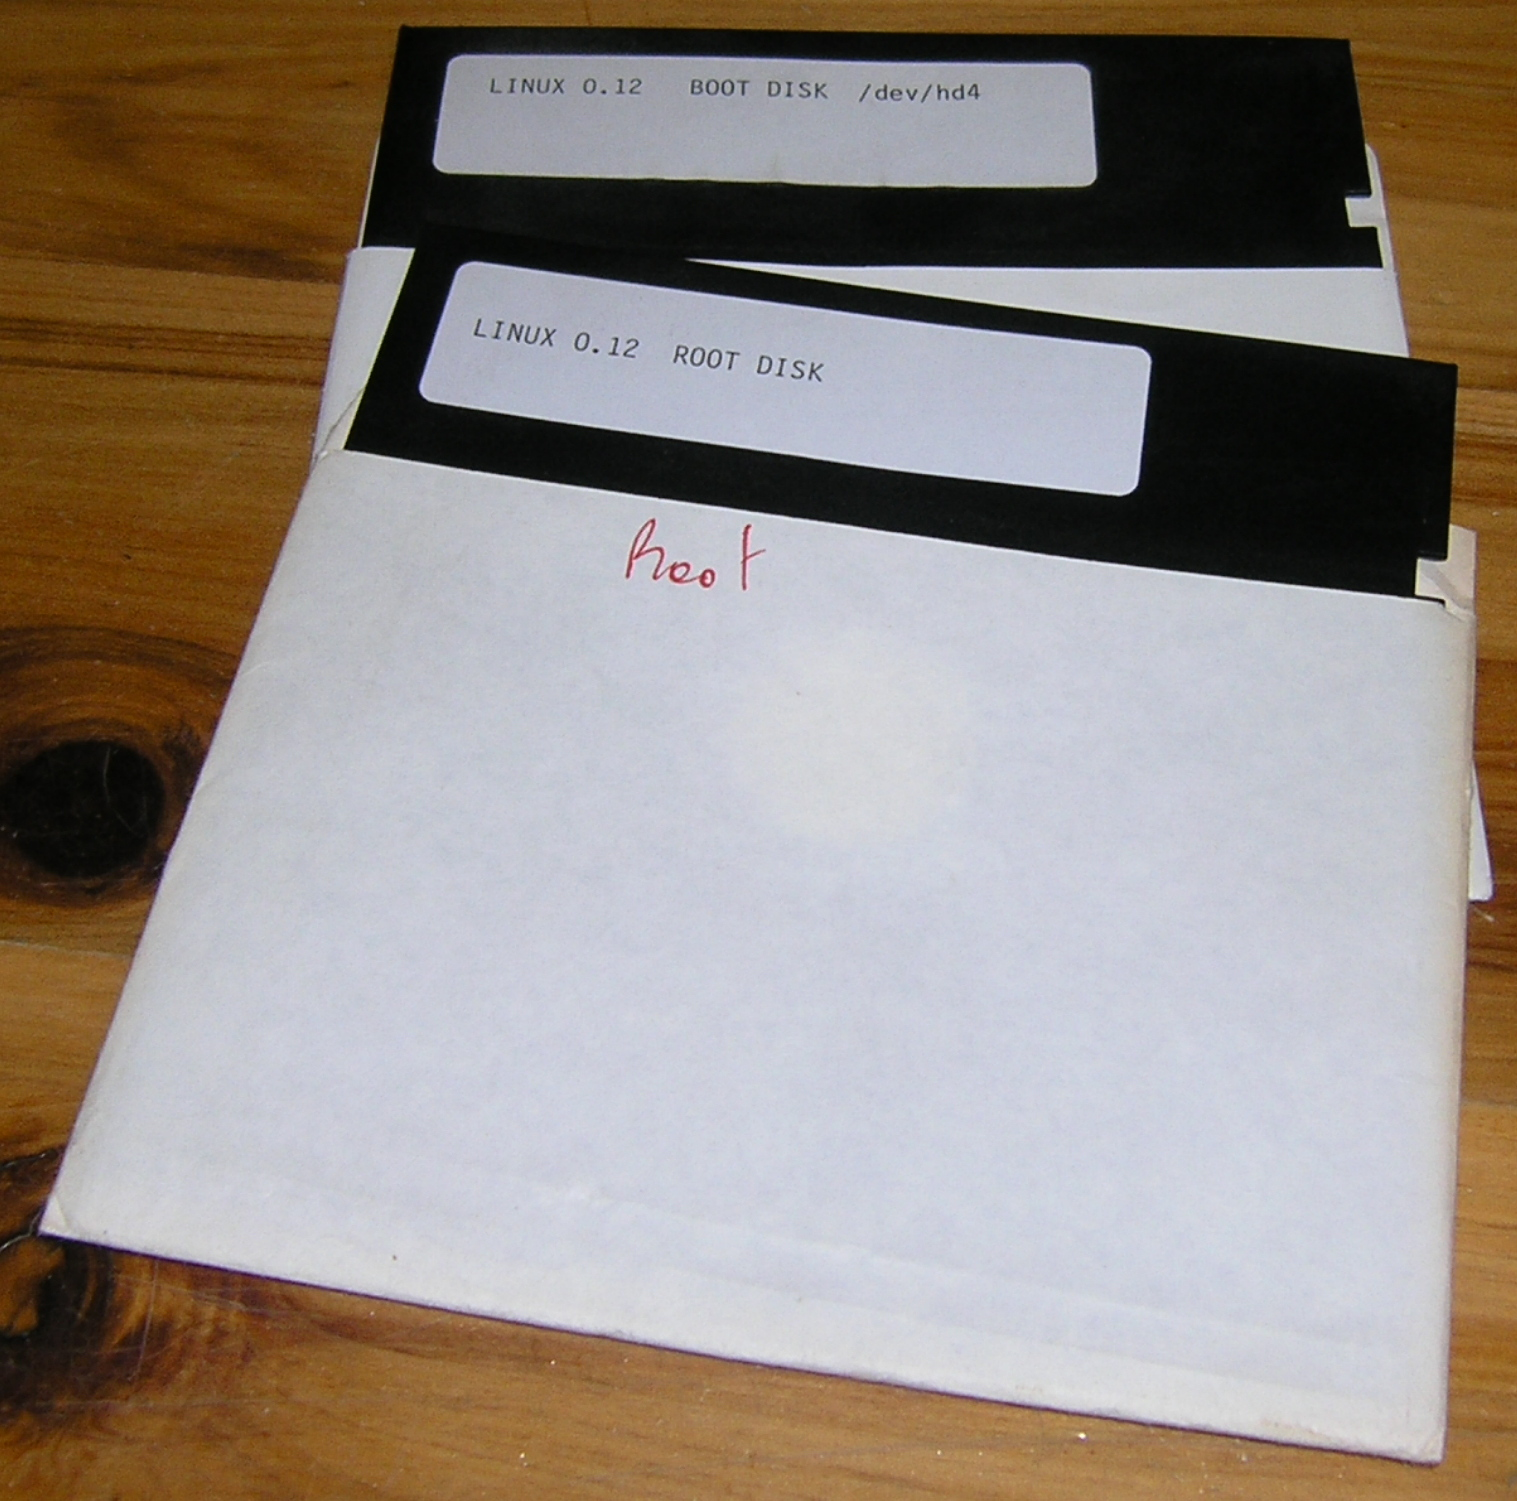
\includegraphics[scale=0.14]{images/Linux_0_12.jpg}
\end{frame}

%------------------------------------------------

\begin{frame}{Le distribuzioni GNU/Linux oggi}
    \centering
    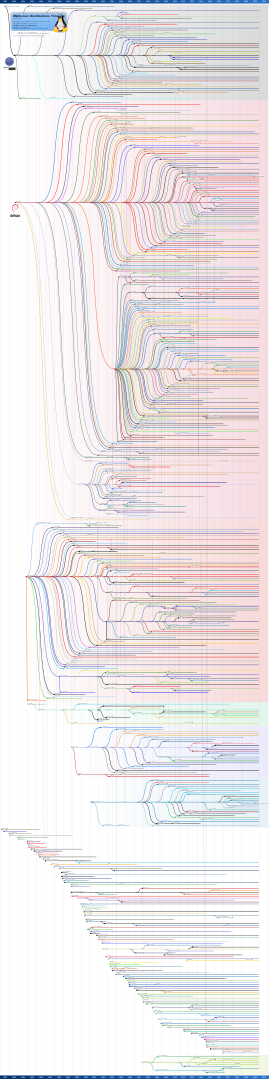
\includegraphics[scale=0.2]{images/Linux_Distribution_Timeline_Dec._2020.svg.png}
\end{frame}

\begin{frame}{Le distribuzioni GNU/Linux oggi}
    \centering
    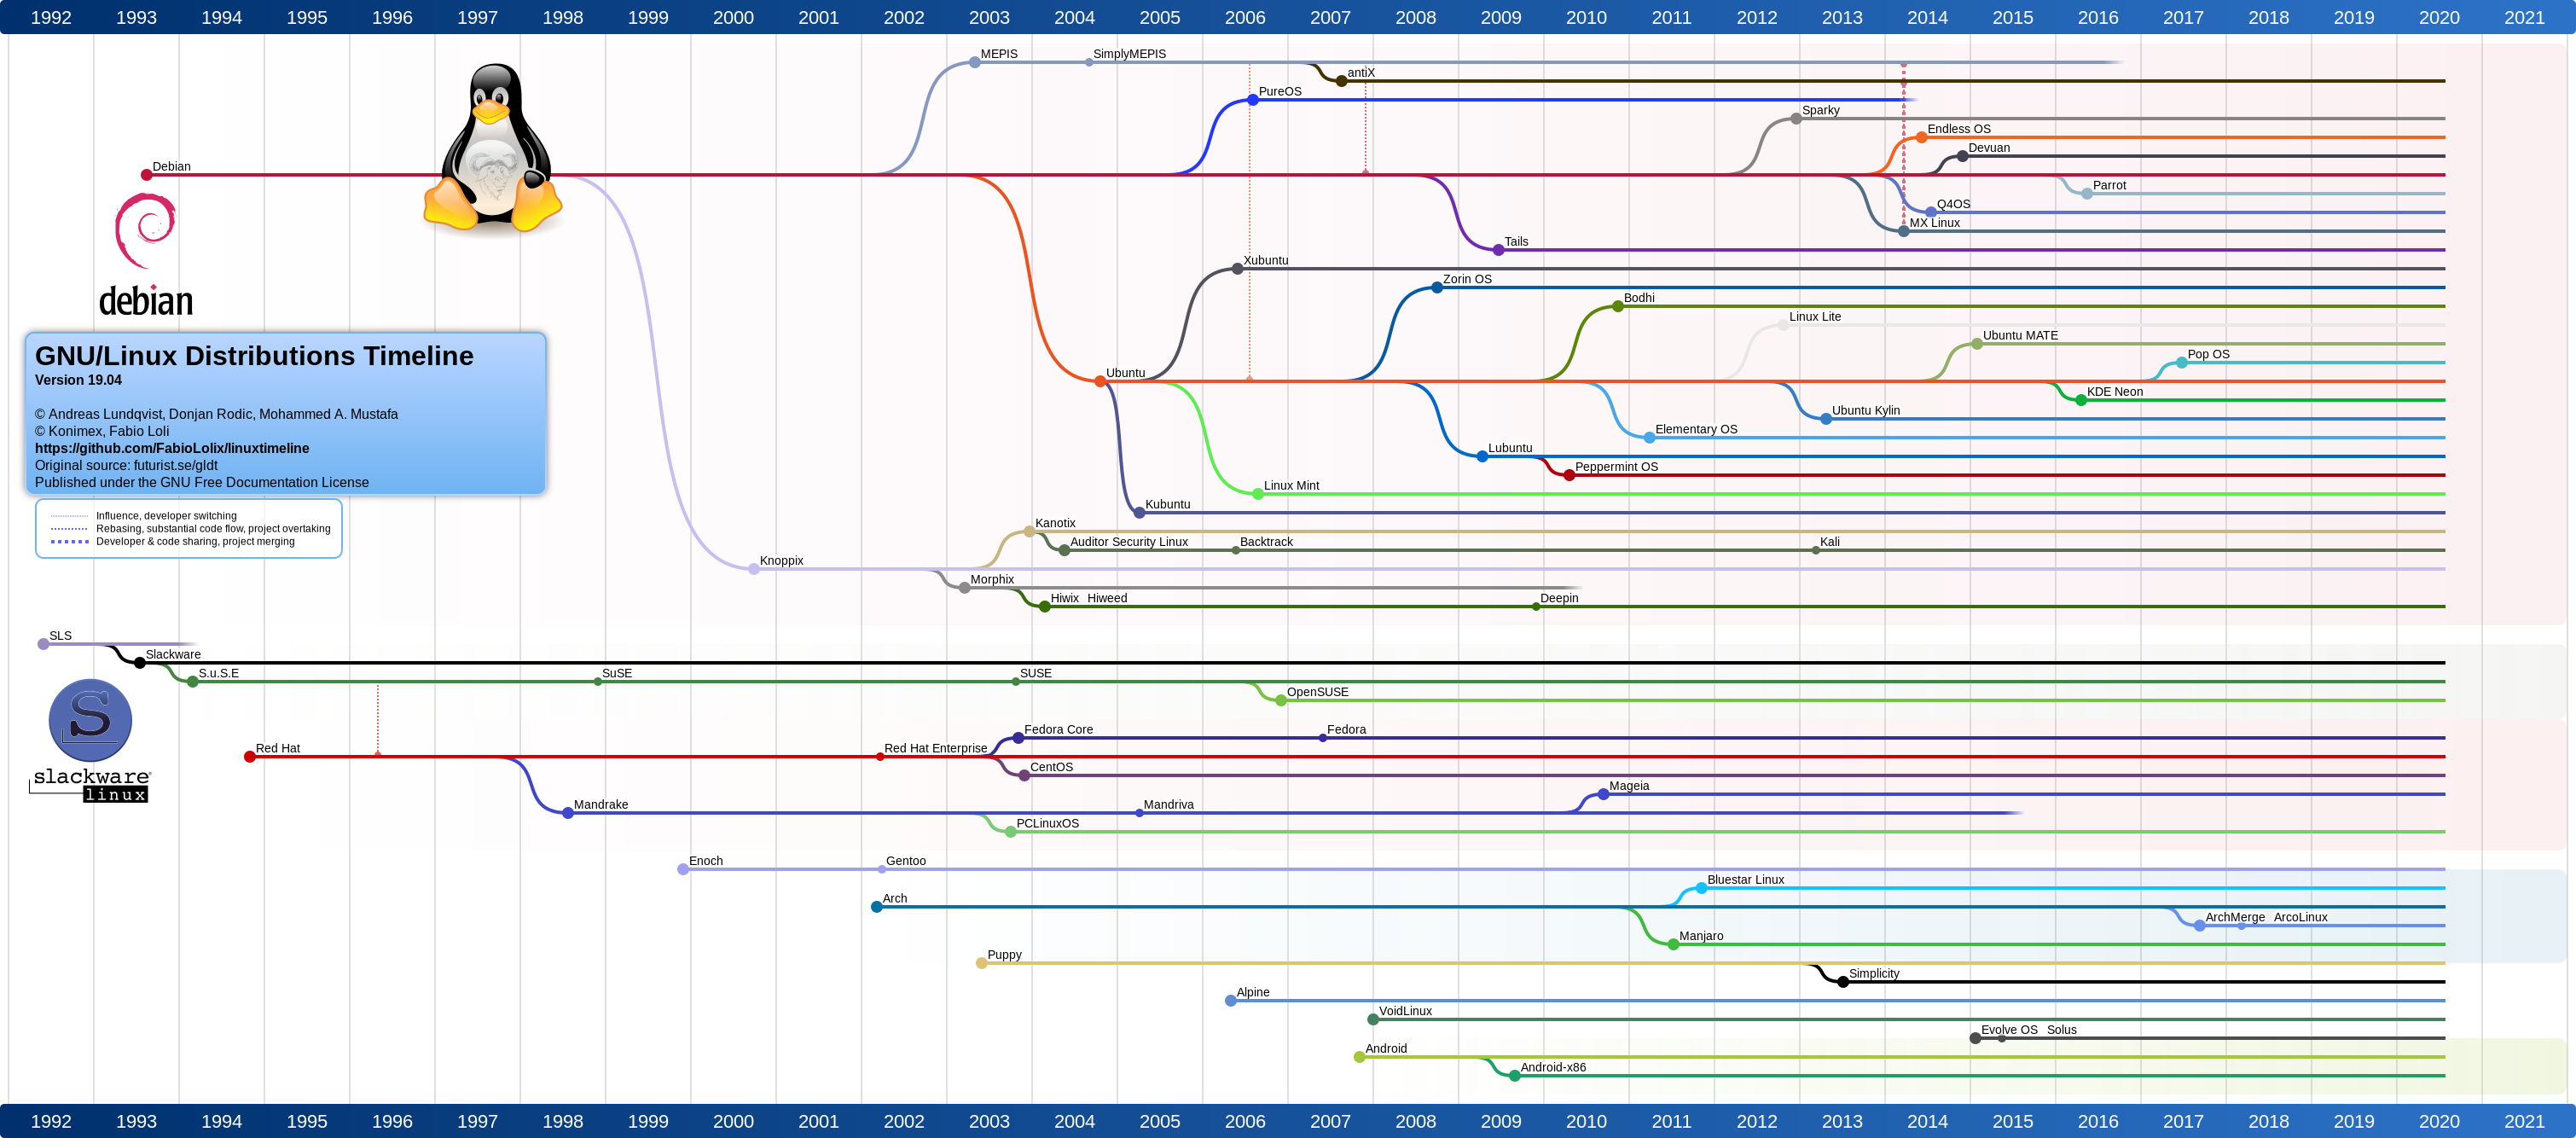
\includegraphics[scale=0.18]{images/aygzaivcbmd51.png}
\end{frame}

\begin{frame}{Le distribuzioni GNU/Linux oggi}
Possiamo suddividere le distribuzioni in GNU/Linux in famiglie:
\begin{itemize}
    \item Debian(Ubuntu, MX Linux, Kali Linux)
    \item Arch Linux(Manjaro, EndeavourOS)
    \item Fedora
    \item Gentoo
    \item ...
\end{itemize}

\end{frame}

%------------------------------------------------
